\section{Hashing}%
\label{sec:hashing}

\begin{frame}
	\frametitle{A hash}
\begin{center}
	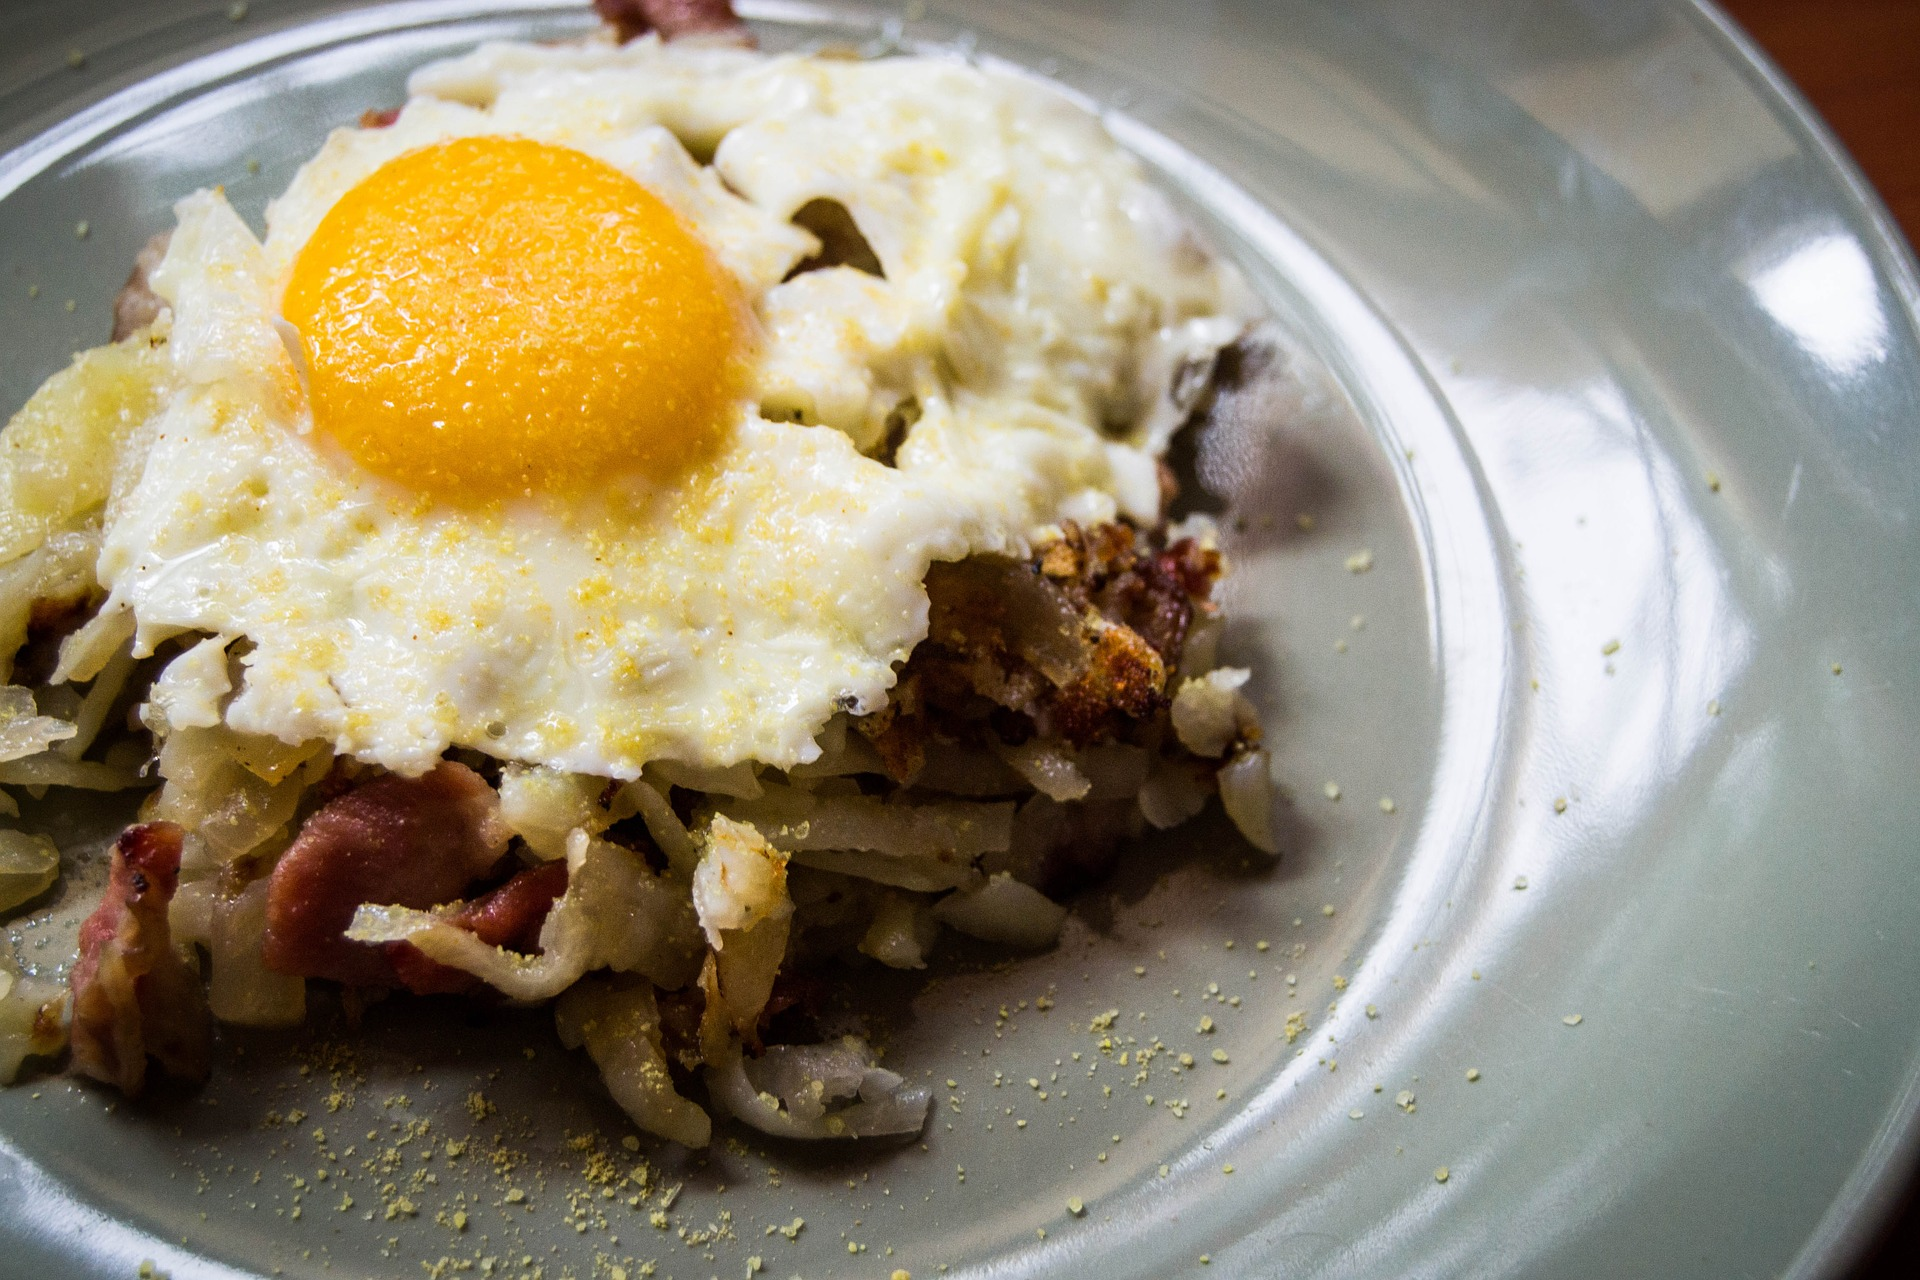
\includegraphics[width=0.6\textwidth]{figures/hash.jpg}\\
	\hspace*{15pt}\hbox{\scriptsize Image By:\thinspace{\itshape ailinder}}
	% https://pixabay.com/photos/hash-eggs-food-meal-potato-plate-1330575/
\end{center}
\end{frame}

\begin{frame}
	\frametitle{Hash functions}
	
		\begin{block}{Hash functions}
			Hash functions map each key $k$ to a an integer in a range $[0, N-1]$ for some $N$.\\
		\end{block}	
		\pause
		\begin{questionblock}{That's easy right?}
			Consider the hash function $f(k) = 1$ for any key $k$.\\
			Is this a hash function for $N=100$?
			\begin{enumerate}[A.]
				\item Yes
				\item No
				\item I don't know
			\end{enumerate}
		\end{questionblock}

		\pause
			\begin{alertblock}{It is...}
				It is a hash function, but a terrible one!\\
				Why?
			\end{alertblock}	
\end{frame}

\begin{frame}
	\frametitle{Hash to determine the index}

	\begin{problemblock}{A hash table}
		We want to use hash functions to map keys to a certain index in a hash table.
	\end{problemblock}
	\pause
	\begin{exampleblock}{Back to hundred-acre woods}
		Take $f(p) = 1$, $f(i) = 3$, $f(g) = 2$, $f(l) = 8$, $f(e) = 5$, $f(t) = 7$.
		\pause
		This would create the hash table:
		\begin{center}
			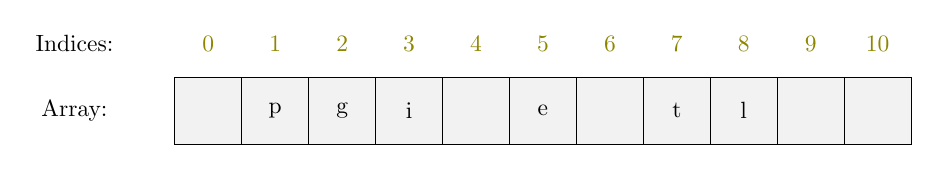
\begin{tikzpicture}[scale=0.85, transform shape]
	\foreach \x/\val in {0/,1/p,2/g,3/i,4/,5/e,6/,7/t,8/l,9/,10/}{
	\node[olive] (index) at (\x,1) {\x};
	\node[draw,rectangle, fill=gray!10, minimum size =1cm] (c) at (\x,0) {\val};
}
\node[] at (-2,1) {Indices:};
\node[] at (-2,0) {Array:};
\end{tikzpicture}

		\end{center}
	\end{exampleblock}	
	\pause
	\begin{alertblock}{The simple mapping}
		But what if we have conflicts? Like by taking $f(k)=1$ for all $k$.
	\end{alertblock}	
\end{frame}

\begin{frame}
	\frametitle{Hashing conflicts}
	\begin{problemblock}{A hash table}
		We want to use hash functions to map keys to a certain index in a hash table.\\
		But what do we do if we have hashing conflicts?
	\end{problemblock}
	\pause
	\begin{exampleblock}{Back to hundred-acre woods}
		Take $f(e) = 1$, $f(y) = 3$, $f(o) = \alert{3}$, $f(r) = 8$.
		\pause
		This would create the hash table:
		\begin{center}
			\begin{tikzpicture}[scale=0.85, transform shape]
	\foreach \x/\val in {0/,1/,2/,3/,4/,5/,6/,7/,8/,9/,10/}{
	\node[olive] (index) at (\x,1) {\x};
	\node[draw,rectangle, fill=gray!10, minimum size =1cm] (\x) at (\x,0) {\val};
}
\node[] at (-2,1) {Indices:};
\node[] at (-2,0) {Array:};

\node[draw,rectangle, fill=gray!10, minimum size =0.5cm] at (1,-1.5) (e) {e};
\node[draw,rectangle, fill=gray!10, minimum size =0.5cm] at (3,-1.5) (A) {y};
\node[draw,rectangle, fill=gray!10, minimum size =0.5cm] at (3,-2.5) (B){o};
\node[draw,rectangle, fill=gray!10, minimum size =0.5cm] at (8,-1.5) (r) {r};
\draw[->, ultra thick] (A) -- (B);
\draw[*->, ultra thick] (1.center) -- (e);
\draw[*->, ultra thick] (3.center) -- (A);
\draw[*->, ultra thick] (8.center) -- (r);
\end{tikzpicture}

		\end{center}
	\end{exampleblock}	
\end{frame}

\begin{frame}
	\frametitle{Hash tables}
	\begin{block}{Hash tables}
		We have an array of a certain capacity.\\
		The hash of a key, determines which \textit{bucket} to use.\\
		\pause
		Every entry could for instance hold a linked-list of values.
	\end{block}		
	\pause
	\begin{columns}
		\column{0.455\textwidth}
			
	\begin{questionblock}{What happens?}
		So for $f(k) = 1$ for all $k$, what is the time complexity of getting the right value out for our key?
		\begin{enumerate}[A.]
			\item $\Theta(1)$
			\item $\Theta(\log n)$
			\item $\Theta(n)$
			\item $\Theta(n^2)$
		\end{enumerate}
	\end{questionblock}
		\column{0.455\textwidth}
			
		\pause
		\begin{answerblock}{Still linear}
			It is still linear time! All end up in a list after all.
		\end{answerblock}
	\end{columns}
\end{frame}

\begin{frame}
	\frametitle{Hash functions: Ideal properties}
	
		\begin{block}{Hash functions}
			Hash functions map each key $k$ to a an integer in a range $[0, N-1]$ for some $N$.\\
			Where ideally:
			\pause
			\begin{itemize}
				\item keys are uniformly distributed over the range.
					\pause
				\item ($a == b) \to (\mathit{hash}(a) == \mathit{hash}(b))$ (it is deterministic).
					\pause
				\item the hash function is `fast' to compute (preferably $O(1)$).
			\end{itemize}

		\end{block}	
			\begin{alertblock}{Rotten to the core}
				This indeed makes $f(k) = 1$ pretty terrible!
			\end{alertblock}	
\end{frame}

\begin{frame}
	\frametitle{Implementing them in Python}
	\only<4->{\framesubtitle{Check for yourself, write a bit of code to count conflicts!}}
		\vspace{-10pt}
	\begin{columns}
		\column{0.555\textwidth}
			\lstinputlisting{code/point.py}
		\pause
		\column{0.555\textwidth}
		\lstinputlisting[firstline=4, lastline=15]{code/point2.py}
	\end{columns}
	\pause
		\vspace{-10pt}
	\begin{questionblock}{Does it improve?}
		Which is better?	
		\vspace{-10pt}
		\begin{multicols}{3}
		\begin{enumerate}[A.]
			\item The left one.
			\item The right one.
			\item I don't know.
		\end{enumerate}
	\end{multicols}
	\end{questionblock}
	\pause
		\vspace{-8pt}
		\begin{answerblock}{It depends!}
			It depends on what kind of points we expect to see!
		\end{answerblock}
\end{frame}
